\documentclass[reqno,12pt]{amsart}

\usepackage[colorlinks=true]{hyperref}
\hypersetup{urlcolor=blue, citecolor=red}

\usepackage{amssymb,graphicx,color}
%\usepackage[english,francais]{babel}
\usepackage[latin1]{inputenc}

%\usepackage[cal=mathpi, frak=mma, scr=rsfs]{mathalfa}
%\usepackage[cal=mtc]{mathalfa}

%The Layout
\setlength{\oddsidemargin}{0pt}
\setlength{\evensidemargin}{0pt}
\setlength{\textheight}{42\baselineskip}
\setlength{\textwidth}{6in}
%\addtolength{\headheight}{0.7in}

\theoremstyle{plain}% default
\newtheorem{thm}{Theorem}[section]
\newtheorem{lem}{Lemma}[section]
\newtheorem{prop}{Proposition}[section]
\newtheorem{cor}{Corollary}[section]
\newtheorem{defs}{Definition}[section]
\newtheorem{prob}{Problem}[section]
\theoremstyle{definition}
\newtheorem{rmk}{Remark}[section]
\newtheorem{fact}{Fact}[section]

\newcommand{\NN}{{\mathbb{N}}}
\newcommand{\ZZ}{{\mathbb{Z}}}
\newcommand{\RR}{{\mathbb{R}}}
\newcommand{\CC}{{\mathbb{C}}}
\newcommand{\QQ}{{\mathbb{Q}}}
\newcommand{\bfu}{\mathbf{u}}
\newcommand{\bfv}{\mathbf{v}}
\newcommand{\bfw}{\mathbf{w}}
\newcommand{\bfe}{\mathbf{e}}
\newcommand{\bfa}{\mathbf{a}}
\newcommand{\bfb}{\mathbf{b}}
\newcommand{\bfg}{\mathbf{g}}
\newcommand{\bff}{\mathbf{f}}
\newcommand{\bfh}{\mathbf{h}}
\newcommand{\bfq}{\mathbf{q}}
\newcommand{\bfx}{\mathbf{x}}
\newcommand{\bfy}{\mathbf{y}}
\newcommand{\bfz}{\mathbf{z}}
\newcommand{\bfr}{\mathbf{r}}
\newcommand{\bfn}{\mathbf{n}}
\newcommand{\bfA}{\mathbf{A}}
\newcommand{\bfB}{\mathbf{B}}
\newcommand{\bfD}{\mathbf{D}}
\newcommand{\bfE}{\mathbf{E}}
\newcommand{\bfI}{\mathbf{I}}
\newcommand{\bfU}{\mathbf{U}}
\newcommand{\bfF}{\mathbf{F}}
\newcommand{\bfR}{\mathbf{R}}
\newcommand{\bfX}{\mathbf{X}}
\newcommand{\bfk}{\mathbf{k}}
\newcommand{\bfj}{\mathbf{j}}
\newcommand{\bfl}{\mathbf{l}}
\newcommand{\bfell}{\boldsymbol{\ell}}
\newcommand{\bfL}{\mathbf{L}}
\newcommand{\bfT}{\mathbf{T}}
\newcommand{\bfM}{\mathbf{M}}
\newcommand{\bfzero}{\mathbf{0}}
\newcommand{\fke}{\mathfrak{e}}
\newcommand{\fkE}{\mathfrak{E}}
\newcommand{\fkf}{\mathfrak{f}}
\newcommand{\fkF}{\mathfrak{F}}
\newcommand{\fkg}{\mathfrak{g}}
\newcommand{\fkG}{\mathfrak{G}}
\newcommand{\fkh}{\mathfrak{h}}
\newcommand{\fkH}{\mathfrak{H}}
\newcommand{\bfcurl}{\mbox{\bf curl}\;}
\newcommand{\bfalpha}{{\boldsymbol{\alpha}}}
\newcommand{\bfvarphi}{\boldsymbol{\varphi}}
\newcommand{\bfPhi}{\boldsymbol{\Phi}}
\newcommand{\bfpsi}{\boldsymbol{\psi}}
\newcommand{\bfxi}{\boldsymbol{\xi}}
\newcommand{\bfnabla}{\boldsymbol{\nabla}}
\newcommand{\bfdelta}{\boldsymbol{\delta}}
\newcommand{\bfomega}{\boldsymbol{\omega}}
\newcommand{\bfsigma}{\boldsymbol{\sigma}}
\newcommand{\bftau}{\boldsymbol{\tau}}
\newcommand{\bfeta}{\boldsymbol{\eta}}
\newcommand{\bfzeta}{\boldsymbol{\zeta}}
\newcommand{\bfkappa}{\boldsymbol{\kappa}}
\newcommand{\bfvarrho}{\boldsymbol{\varrho}}
\newcommand{\bfchi}{\boldsymbol{\chi}}
\newcommand{\define}{\stackrel{\mathrm{def}}{=}}
\newcommand{\Ccal}{{\mathcal C}}
\newcommand{\Acal}{{\mathcal A}}
\newcommand{\Bcal}{{\mathcal B}}
\newcommand{\Fcal}{{\mathcal F}}
\newcommand{\Scal}{{\mathcal S}}
\newcommand{\Ncal}{{\mathcal N}}
\newcommand{\Rcal}{{\mathcal R}}
\newcommand{\Qcal}{{\mathcal Q}}
\newcommand{\Gcal}{{\mathcal G}}
\newcommand{\Kcal}{{\mathcal K}}
\newcommand{\Xcal}{{\mathcal X}}
\newcommand{\Ycal}{{\mathcal Y}}
\newcommand{\Zcal}{{\mathcal Z}}
\newcommand{\Vcal}{{\mathcal V}}
\newcommand{\Wcal}{{\mathcal W}}
\newcommand{\per}{{\mathrm{per}}}
\newcommand{\ch}{{\mathrm{ch}}}
\newcommand{\loc}{{\mathrm{loc}}}
\newcommand{\zave}[1]{\dot{#1}}
\newcommand{\Ecal}{{\mathcal E}}
\newcommand{\Mcal}{{\mathcal M}}
\newcommand{\Pcal}{{\mathcal P}}
\newcommand{\Dcal}{{\mathcal D}}
\newcommand{\Tcal}{{\mathcal T}}
\newcommand{\Ucal}{{\mathcal U}}
\newcommand{\Lcal}{{\mathcal L}}
\newcommand{\Ocal}{{\mathcal O}}
\newcommand{\Gr}{\mathrm{G}}
\newcommand{\Rey}{\mathrm{Re}}
\newcommand{\rmD}{\mathrm{D}}
\newcommand{\rmH}{\mathrm{H}}
\newcommand{\rmP}{\mathrm{P}}
\newcommand{\rmS}{\mathrm{S}}
\newcommand{\rmKo}{\mathrm{Ko}}
\newcommand{\rmKr}{\mathrm{Kr}}
\newcommand{\rmd}{\mathrm{d}}
\newcommand{\rmw}{\mathrm{w}}
\newcommand{\rmv}{\mathrm{v}}
\newcommand{\rmreg}{\mathrm{reg}}
\newcommand{\rmb}{\mathrm{b}}
\newcommand{\rmg}{\mathrm{g}}
\newcommand{\rmc}{\mathrm{c}}
\newcommand{\rmr}{\mathrm{r}}
\newcommand{\rms}{\mathrm{s}}
\newcommand{\sfA}{\mathsf{A}}
\newcommand{\sfD}{\mathsf{D}}
\newcommand{\sfT}{\mathsf{T}}
\newcommand{\sfI}{\mathsf{I}}
\newcommand{\sfJ}{\mathsf{J}}
\newcommand{\sfS}{\mathsf{S}}
\newcommand{\sfsigma}{\mathsf{\sigma}}
\newcommand{\sftau}{\mathsf{\tau}}
\newcommand{\sgn}{\operatorname{sgn}}
\newcommand{\Id}{\operatorname{Id}}
\newcommand{\tr}{{\operatorname{tr}}}
\newcommand{\supp}{\operatorname*{supp}}
\newcommand{\Tr}{\operatorname{Tr}}
\newcommand{\Cyl}{\operatorname{\mathcal{C}_{yl}}}
\newcommand{\Syl}{\operatorname{\mathcal{S}_{yl}}}
\newcommand{\nse}{{\operatorname{nse}}}
\newcommand{\cyl}{{\operatorname{cyl}}}
\newcommand{\sss}{{\operatorname{sss}}}
\newcommand{\fpsss}{{\operatorname{fpsss}}}
\newcommand{\wsss}{{\operatorname{wsss}}}
\newcommand{\tasss}{{\operatorname{tasss}}}
\newcommand{\inv}{{\operatorname{inv}}}
\newcommand{\Linv}{{\operatorname{L-inv}}}
\newcommand{\Einv}{{\operatorname{E-inv}}}
\newcommand{\sinv}{{\operatorname{\sigma-inv}}}
\newcommand{\Piinv}{{\operatorname{\Pi-inv}}}
\newcommand{\average}[1]{\langle{#1}\rangle}
\newcommand{\dual}[1]{\langle{#1}\rangle}
\newcommand{\inner}[1]{({#1})}
\newcommand{\dinner}[1]{(\!({#1})\!)}
\newcommand{\Lim}{\operatorname*{\textsc{Lim}}_{T\rightarrow \infty}}
\newcommand{\co}{\operatorname*{\text{co}}}
\newcommand{\paratitle}[1]{\vspace{\baselineskip} \noindent \emph{{#1}}}
%\newcommand{\comment}[1]{\textcolor{red}{\framebox{\parbox{0.9\textwidth}{\textbf{#1}}}}}
\newcommand{\comment}[1]{\textcolor{red}{\textbf{#1}}}
\newcommand{\doshow}[1]{#1}
\newcommand{\dontshow}[1]{}
\newcommand{\extra}[1]{\dontshow{#1}} % use \show to show the extra stuff or \donotshow not to show it

%\mathchardef\mhyphen="2D

\renewcommand{\subjclassname}{$2020$ Mathematics Subject Classification}

\renewcommand{\theenumi}{\roman{enumi}}

\begin{document}
\numberwithin{equation}{section}

% Article info

\title[Strong order 1 convergence of Euler-Maruyama for Random ODEs]{Conditions for the strong order 1 convergence of the Euler-Maruyama approximation for Random Ordinary Differential Equations}

\author[R. M. S. Rosa]{Ricardo M. S. Rosa}

\author[P. E. Kloeden]{Peter E. Kloeden}

\address[Ricardo M. S. Rosa]{Instituto de Matem\'atica, Universidade Federal do Rio de Janeiro, Brazil}
\address[Peter E. Kloeden]{Mathematics Department, University of Tubingen, Germany}

\email[R. M. S. Rosa]{rrosa@im.ufrj.br}
\email[P. E. Kloeden]{kloeden@math.uni-frankfurt.de}

\date{\today}

%\thanks{This work was partly supported by the CNPq, Bras\'{\i}lia, Brazil and by the NSF grant ???.}

\subjclass[2000]{76D05, 76D06, 35Q30, 37L99}
\keywords{random ordinary differential equations, Euler-Maruyama method, strong convergence, It\^o process, point process}.

\begin{abstract}
It is well known that the Euler-Maruyama method of approximating a random ordinary differential equation $\mathrm{d}X_t/\mathrm{d}t = f(t, X_t, Y_t)$ driven by a stochastic process $\{Y_t\}_t$ with $\theta$-H\"older sample paths is estimated to be of strong order $\theta$ with respect to the time step, provided $f=f(t, x, w)$ is sufficiently regular. Here, we show that, in common situations, it is possible to exploit ``hidden'' conditions on the noise and prove that the strong convergence is actually of order 1, regardless of much regularity on the sample paths. This applies to It\^o process noises (such as Wiener, Orstein-Uhlenbeck, and Geometric Brownian process), which are H\"older continuous, and to point processes (such as Poisson point processes and Hawkes self-exciting processes), which are not even continuous and have jump-type discontinuities. The order 1 convergence follows from not estimating directly the local error, but, instead, adding up the local steps and estimating the compound error. In the case of an It\^o noise, the compound error is then estimated via It\^o formula and the It\^o isometry. In the case of a point process, a monotonic bound is exploited. We HOPEFULLY complement the result by giving examples where some of the conditions are not met and the order of convergence seems indeed to be less than 1.
\end{abstract}

\maketitle

\section{Introduction}

Consider the following initial value problem for a \textbf{random ordinary differential equation (RODE)}:
\begin{equation}
  \label{rodeeq}
  \begin{cases}
    \displaystyle \frac{\mathrm{d}X_t}{\mathrm{d} t} = f(t, X_t, Y_t), \qquad 0 \leq t \leq T, \\
    \left. X_t \right|_{t = 0} = X_0,
  \end{cases}
\end{equation}
where the noise $\{Y_t\}_{t\in I}$ is a real stochastic process. The sample space is denoted by $\Omega$. We also treat systems of random ordinary equations, as discussed later in the article, but we start with the scalar case, in order to present the main ideas.

The Euler-Maruyama method for solving this initial value problem on the time interval $I = [0, T]$ consists in approximating the solution on a uniform time mesh $t_j = j\Delta t$, $j = 0, \ldots, N$, with fixed time step $\Delta t = T/N$, for a given $N\in \mathbb{N}$. In such a mesh, the Euler-Maruyama scheme takes the form
\begin{equation}
  \label{emscheme}
  X_{t_j}^N = X_{t_{j-1}}^N + \Delta t f(t_{j-1}, X_{t_{j-1}}^N, Y_{t_{j-1}}), \qquad j = 1, \ldots, N,
\end{equation}
with the initial condition
\begin{equation}
  \label{iccondition}
  X_0^N = X_0.
\end{equation}
Notice both $\Delta t = \Delta t_N = T/N$ and $t_j = t_j^N = j\Delta t_N = jT/N$ depend on $N$, but we sometimes do not make this dependency explicit, for the sake of notational simplicity.

When the noise $\{Y_t\}_{t\in I}$ has $\theta$-H\"older continuous sample paths, it can be show, under further suitable conditions, that the Euler-Maruyama scheme converges strongly with order $\theta$ with the time step, i.e. there exists $C > 0$ such that
\begin{equation}
    \max_{j=0, \ldots, N}\mathbb{E}\left[ \left| X_{t_j} - X_{t_j}^N \right| \right] \leq C \Delta t_N^\theta, \qquad \forall N \in \mathbb{N},
\end{equation}
where $\mathbb{E}[\cdot]$ indicates the expectation of a random variable on $\Omega$ (see \cite{}).

Our aim is to show that, in many classical examples, it is possible to exploit further ``hidden'' conditions that yield in fact a strong order 1 convergence, even when the sample paths are still H\"older continuous or have jump discontinuities. This is the case, for instance, when the noise is an It\^o noise, and when the equation is semi-separable and the noise is a point process.

More precisely, for the semi-separable case, we assume $f$ is of the form $f(t, x, y) = a(t, y)h(t, x) + b(t, y)$, so the RODE takes the form
\begin{equation}
    \label{semiseparablerodeeq}
    \begin{cases}
        \displaystyle \frac{\mathrm{d}X_t}{\mathrm{d} t} = a(t, Y_t) h(X_t) + b(t, Y_t), \qquad 0 \leq t \leq T, \\
        \left. X_t \right|_{t = 0} = X_0.
    \end{cases}
\end{equation}
In this case, we assume the processes $\{a(t, Y_t)\}_{t\in I}$ and $\{b(t, Y_t)\}_{t\in I}$ have their steps bounded monotonically, which typically happens for point processes, i.e.
\[
a(t+\tau, Y_{t+\tau}) - a(t, Y_t) \leq A_t.
\]

We show that if \textcolor{red}{describe the conditions needed in Section \ref{secmonotonicbound}}, then 

For the It\^o noise case, we consider a general equation of the form \eqref{rodeeq},
\begin{equation}
    \begin{cases}
      \displaystyle \frac{\mathrm{d}X_t}{\mathrm{d} t} = f(t, X_t, Y_t), \qquad 0 \leq t \leq T, \\
      \left. X_t \right|_{t = 0} = X_0,
    \end{cases}
  \end{equation}
with a noise defined as an \textbf{It\^o process} $\{Y_t\}_{t\geq 0}$, satisfying
\begin{equation}
  \mathrm{d}Y_t = A_t \;\mathrm{d}t + B_t \;\mathrm{d}W_t,
\end{equation}
We are not solving for $Y_t$, nor approximating it numerically, otherwise we would actually need to consider a system of stochastic differential equations. Instead, we assume it is a known process that can be computed analytically, such as a Wiener process, an Orstein-Uhlenbeck process, or a geometric Brownian motion. With those in mind, we allow $A_t$ and $B_t$ to be originally given in terms of $\{W_t\}_{t\geq 0}$ and $\{Y_t\}_{t\geq 0}$.

In the case that $f=f(t, x, y)$ is twice continuously differentiable, the It\^o formula yields
\begin{multline}
  \mathrm{d}f(t, x, Y_t) = \left(\partial_t f(t, x, Y_t) + A_t \partial_y f(t, x, Y_t)  + \frac{B_t^2}{2}\partial_{yy}f(t, x, Y_t) \right) \;\mathrm{d}t \\ + B_t \partial_y f(t, x, Y_t)\;\mathrm{d}W_t.
\end{multline}

We show that, if the expectations of $\{A_t\}_t$ and $\{B_t\}_t$ are uniformly bounded in time on $[0, T]$ and $\partial_t f$, $\partial_x f$, $\partial_y f$, and $\partial_{yy}f$ are uniformly bounded on $[0, T]\times \mathbb{R}\times \mathbb{R}$, then the Euler-Maruyama method is of strong order 1, i.e. there exists $C>0$ such that
\begin{equation}
    \max_{j=0, \ldots, N}\mathbb{E}\left[ \left| X_{t_j} - X_{t_j}^N \right| \right] \leq C \Delta t_N, \qquad \forall N \in \mathbb{N},
\end{equation}
where $\mathbb{E}[\cdot]$ indicates the expectation of a random variable on $\Omega$ (see Theorem \ref{EMstrongorder1}).

We summarize here the main tricks we use to accomplish such error estimate:
\begin{enumerate}
  \item We assume the noise is an It\^o process, so we can use the It\^o isometry at some point;
  \item We use the It\^o formula to separate the most problematic/rough part of the noise;
  \item We do not estimate this problematic term locally at each time step;
  \item Instead, we add up the difference equation for the time steps and write the error in terms of a time integral of this rough part of the noise;
  \item We then use the It\^o isometry to estimate this integral term by $\Delta t$;
\end{enumerate}

In order to make the main idea clear cut, here are the options we have for estimating the rough part of the noise:
\begin{enumerate}
  \item If the local error $e_j$ of the rough part of the noise, at the $j$th time step, is bounded as
    $$
    \mathbb{E}[|e_j|] \lesssim \Delta t^{3/2},
    $$
    as usual for a $1/2$-H\"older noise, then adding them up leads to 
    $$
      \sum \mathbb{E}[|e_j|] \lesssim N\Delta t^{3/2} = T\Delta t^{1/2}.
    $$
    \item If we use the It\^o isometry locally, we still get the local error as
    $$
      \mathbb{E}[|e_j|] \leq \mathbb{E}[|e_j|^2]^{1/2} \lesssim \left(\Delta t^{2(3/2)} \right)^{1/2} = \Delta t^{3/2},
    $$
    and adding that up still leads to an error of order $\Delta t^{\theta}$.
    \item If, instead, we first add the terms up, then $\sum e_j$ becomes an integral over $[0, T]$ with respect to the Wiener noise, so that we can use the It\^o isometry on the added up term and obtain
    \begin{multline*}
      \mathbb{E}\left[ \left| \sum e_j \right| \right] \lesssim \left(\mathbb{E}\left[ \left| \sum e_j \right|^2 \right]\right)^{1/2} = \left( \sum \mathbb{E}[|e_j|^2] \right)^{1/2} \\
      = \left( \sum \Delta t^3 \right)^{1/2} = \left( \Delta t^2 \right)^{1/2} = \Delta t.
    \end{multline*}
    and we finally get the error to be of order 1.
\end{enumerate}

\section{Pathwise solution}
\label{secpathwisesolution}

We consider a function $f=f(t, x, y)$ defined on $[0, T]\times \mathbb{R}\times\mathbb{R}$ and a real-valued stochastic process $\{Y_t\}_{t\in I}$.

We assume that $f$ is globally Lipschitz continuous on $x$, uniformly in $t$ and $y$, i.e.
There exists $L_x > 0$ such that
    \begin{equation}
        \label{Lxassumptionbasic}
        |f(t, x_1, y) - f(t, x_2, y)| \leq L_x |x_1 - x_2|, \qquad \forall t \in [0, T], \;\forall x_1, x_2, y\in\mathbb{R}.
    \end{equation}
We also assume that $(t, x) \mapsto f(t, x, Y_t)$ satisfies the \emph{Carath\'eodory conditions.} More precisely, we assume that
\begin{enumerate}
    \item The mapping $x \mapsto f(t, x, y)$ is continuous on $x\in \mathbb{R}$, for almost every $(t, y)\in I\times \mathbb{R}$;
    \item The mapping $t \mapsto f(t, x, Y_t)$ is Lebesgue measurable in $t\in [0, T]$, for each $x\in \mathbb{R}$ and each sample path $t \mapsto Y_t(\omega)$;
    \item The bound $|f(t, x, Y_t)| \leq m(t, R)$ holds for all $t\in I$ and all $|x| \leq R$, where $t\mapsto m(t, R)$ is absolutely continuous on $t\in [0, T]$, for each $R>0$.
\end{enumerate}

Under these assumptions, the integral equation
\begin{equation}
    \label{integralrodeform}
    X_t = X_0 + \int_0^t f(s, X_s, Y_s) \;\mathrm{d}s
\end{equation}
has a unique solution, for each sample $X_0 = X_0(\omega)$ of the initial condition and sample path $t\mapsto Y_t(\omega)$ of the noise process.

The mapping $(t, \omega) \mapsto X_t(\omega)$ is measurable since it can be seen as the pointwise limit of the Picard iterations
\[
X_t^n = X_0 + \int_0^t f(s, X_s^{n-1}, Y_s)\;\mathrm{d}s, \qquad n \in \mathbb{N}, \quad X_t^0 = X_0,
\]
which are, themselves, measurable.

This yields a well-defined stochastic process $\{X_t\}_{t\in I}$ as a pathwise solution of the RODE \eqref{rodeeq}.

When $f=f(t, x, y)$ is continuous on all three variables, as well as uniformly globally Lipscthiz continuous on $x$, and the sample paths of $\{Y_t\}_{t\geq 0}$ are continuous, then the integrand in \eqref{integralrodeform} is continuous on $t$ and the integral becomes a Riemann integral.

\section{Integral formula for the global pathwise error}

In this section, we derive the following integral formula for the global error:
\begin{lem}
    Suppose $f=f(t, x, y)$ satisfies the Carath\'eodory conditions in Section \ref{secpathwisesolution}. Then, the Euler-Maruyama approximation \eqref{emscheme} for any pathwise solution of the random ordinary differential equation \eqref{rodeeq} satisfies the global error formula
    \begin{equation}
        \label{globalerrorintegralformula}
        \begin{aligned}
            X_{t_j} - X_{t_j}^N & = X_0 - X_0^N \\
            & \qquad + \int_0^{t_j} \left( f(s, X_s, Y_s) - f(s, X_{\tau^N(s)}, Y_s) \right)\;\mathrm{d}s  \\ 
            & \qquad + \int_{0}^{t_j} \left( f(s, X_{\tau^N(s)}, Y_s) - f(s, X_{\tau^N(s)}^N, Y_s) \right)\;\mathrm{d}s \\
            & \qquad + \int_0^{t_j} \left( f(s, X_{\tau^N(s)}^N, Y_s) - f(\tau^N(s), X_{\tau^N(s)}^N, Y_{\tau^N(s)}) \right)\;\mathrm{d}s,
        \end{aligned}
    \end{equation}
    for $j = 1, \ldots, N,$ where $\tau^N$ is the piecewise constant jump function along the time mesh:
    \begin{equation}
        \label{tauNt}
        \tau^N(t) = \max_j\{j\Delta t_N; \; j\Delta t_N \leq t\} = \left[\frac{t}{\Delta t_N}\right]\Delta t_N = \left[\frac{tN}{T}\right]\frac{T}{N}.
    \end{equation}
\end{lem}

\begin{proof}
    Under the Carath\'eodory conditions, the solutions of \eqref{rodeeq} are pathwise solutions in the sense of \eqref{integralrodeform}. With that in mind, we first obtain an expression for a single time step, from time $t_{j-1}$ to $t_j = t_{j-1} + \Delta t$.
    
    For notational simplicity, we momentarily write $t = t_{j-1}$ and $\tau = \Delta t_N$, so that $t_j = t + \tau$. The exact pathwise solution satisfies
    $$
    X_{t + \tau} = X_t + \int_t^{t + \tau} f(s, X_s, Y_s) \;\mathrm{d}s.
    $$
    The Euler-Maruyama step is given by
    $$
    X_{t+\tau}^N = X_t^N + \tau f(t, X_t^N, Y_t).
    $$
    Subtracting, we obtain
    $$
    X_{t + \tau} - X_{t + \tau}^N = X_t - X_t^N + \int_t^{t + \tau} \left( f(s, X_s, Y_s) - f(t, X_t^N, Y_t) \right)\;\mathrm{d}s.
    $$

    We arrange the integrand as
    \begin{align*}
    f(s, X_s, Y_s) - f(t, X_t^N, Y_t) = & f(s, X_s, Y_s) - f(s, X_t, Y_s) \\ 
    & + f(s, X_t, Y_s) - f(s, X_t^N, Y_s) \\
    & + f(s, X_t^N, Y_s) - f(t, X_t^N, Y_t).
    \end{align*}

    This yields
    \begin{align*}
        X_{t + \tau} - X_{t + \tau}^N  = & X_t - X_t^N \\
        = &  \int_t^{t + \tau} \left( f(s, X_s, Y_s) - f(s, X_t, Y_s) \right)\;\mathrm{d}s \\ 
        & + \int_t^{t + \tau} \left( f(s, X_t, Y_s) - f(s, X_t^N, Y_s) \right)\;\mathrm{d}s \\
        & + \int_t^{t + \tau} \left( f(s, X_t^N, Y_s) - f(t, X_t^N, Y_t) \right)\;\mathrm{d}s.
    \end{align*}

    Going back to the notation $t = t_{j-1}$ and $t + \tau = t_j$, the above identity reads
    \begin{equation}
        \label{singlestep}
        \begin{aligned}
            X_{t_j} - X_{t_j}^N  = & X_{t_{j-1}} - X_{t_{j-1}}^N \\
            = &  \int_{t_{j-1}}^{t_j} \left( f(s, X_s, Y_s) - f(s, X_{t_{j-1}}, Y_s) \right)\;\mathrm{d}s \\ 
            & + \int_{t_{j-1}}^{t_j} \left( f(s, X_{t_{j-1}}, Y_s) - f(s, X_{t_{j-1}}^N, Y_s) \right)\;\mathrm{d}s \\
            & + \int_{t_{j-1}}^{t_j} \left( f(s, X_{t_{j-1}}^N, Y_s) - f(t_{j-1}, X_{t_{j-1}}^N, Y_{t_{j-1}}) \right)\;\mathrm{d}s.
        \end{aligned}
    \end{equation}

    Now we iterate the time steps \eqref{singlestep} to find that
    \begin{align*}
        X_{t_j} - X_{t_j}^N & = X_0 - X_0^N \\
        & \qquad + \sum_{i=1}^{j} \left(\int_{t_{i-1}}^{t_i} \left( f(s, X_s, Y_s) - f(s, X_{t_{i}}, Y_s) \right)\;\mathrm{d}s \right. \\ 
        & \qquad + \int_{t_{i-1}}^{t_i} \left( f(s, X_{t_{i-1}}, Y_s) - f(s, X_{t_{i-1}}^N, Y_s) \right)\;\mathrm{d}s \\
        & \qquad \left. + \int_{t_{i-1}}^{t_i} \left( f(s, X_{t_{i-1}}^N, Y_s) - f(t_{i-1}, X_{t_{i-1}}^N, Y_{t_{i-1}}) \right)\;\mathrm{d}s \right).
    \end{align*}

    Using the jump function $\tau^N$, we may rewrite the above expression as in \eqref{globalerrorintegralformula}.
\end{proof}

\section{Basic estimate}

Here we derive an estimate, under minimal hypotheses, that will be the basis for the estimates in specific cases.

\begin{lem}
    \label{lembasicestimate}
    Suppose $f=f(t, x, y)$ satisfies the Carath\'eodory conditions in Section \ref{secpathwisesolution} and is uniformly globally Lipschitz continuous on $x$ with Lipschitz constant $L_x$, as in \eqref{Lxassumptionbasic}. Then, the global error \eqref{globalerrorintegralformula} is estimated as
    \begin{equation}
        \label{Etjbasicbound}
        \begin{aligned}
            |X_{t_j} - X_{t_j}^N| & \leq \left( |X_0 - X_0^N| + L_x \int_0^{t_j} |X_s - X_{\tau^N(s)}| \;\mathrm{d}s \right. \\
            & \qquad \left. \left|\int_0^{t_j} \left( f(s, X_{\tau^N(s)}^N, Y_s) - f(\tau^N(s), X_{\tau^N(s)}^N, Y_{\tau^N(s)}) \right)\;\mathrm{d}s\right|\right) e^{L_x t_j}.
        \end{aligned}
    \end{equation}
    for $j=1, \ldots, N$, where $\tau^N$ is given by \eqref{tauNt}.
\end{lem}

\begin{proof}
    We estimate the first two integrals in \eqref{globalerrorintegralformula}. For the first one, we use \eqref{Lxassumptionbasic}, so that
    $$
        |f(s, X_s, Y_s) - f(s, X_t, Y_s)| \leq L_x |X_s - X_t|,
    $$
    for $t, s \in [0, T]$, and, in particular, for $t = \tau^N(s)$. Hence,
    $$
        \left|\int_0^{t_j} \left( f(s, X_s, Y_s) - f(s, X_{\tau^N(s)}, Y_s) \right)\;\mathrm{d}s \right| \leq L_x \int_0^{t_j} |X_s - X_{\tau^N(s)}| \;\mathrm{d}s.
    $$
    
    For the second term, we use again \eqref{Lxassumption}, so that
    $$
        |f(s, X_t, Y_s) - f(s, X_t^N, Y_s)| \leq L_x |X_t - X_t^N|,
    $$
    again for any $t, s \in [0, T]$, and, in particular, for $t = \tau^N(s)$. Hence,
    \begin{multline*}
        \left|\int_0^{t_j} \left( f(s, X_{\tau^N(s)}, Y_s) - f(s, X_{\tau^N(s)}^N, Y_s) \right)\;\mathrm{d}s \right| \leq L_x \int_0^{t_j} |X_{\tau^N(s)} - X_{\tau^N(s)}^N| \;\mathrm{d}s \\
        \leq L_x\sum_{i=0}^{j-1} |X_{t_i} - X_{t_i}^N|\Delta t.
    \end{multline*}
    
    With these two estimates, we bound \eqref{globalerrorintegralformula} as
    \begin{align*}
        |X_{t_j} - X_{t_j}^N| & \leq |X_0 - X_0^N| \\
        & \qquad + L_x \int_0^{t_j} |X_s - X_{\tau^N(s)}| \;\mathrm{d}s  \\ 
        & \qquad + L_x\sum_{i=0}^{j-1} |X_{t_i} - X_{t_i}^N|\Delta t \\
        & \qquad + \left|\int_0^{t_j} \left( f(s, X_{\tau^N(s)}^N, Y_s) - f(\tau^N(s), X_{\tau^N(s)}^N, Y_{\tau^N(s)}) \right)\;\mathrm{d}s\right|.
    \end{align*}
    Using the discrete version of the Gronwall Lemma, we prove \eqref{Etjbasicbound}.
\end{proof}

The first term in the right hand side of \eqref{Etjbasicbound} usually vanishes since in general we take $X_0^N = X_0$, but it suffices to assume that
\begin{equation}
    \mathbb{E}[|X_0^N - X_0|] \leq C_0 \Delta t_N, \qquad N\in \mathbb{N},
\end{equation}
for some constant $C_0$, which is useful for lower order approximations or for the discretization of random partial differential equations.

The third term in \eqref{Etjbasicbound} is the more delicate one that will be handled differently in the next sections.

As for the second term, that just concerns the solution itself, not the approximation, and for that we use the following simple but useful general result.

\begin{lem}
    \label{estimatesecondterminglobalerror}
    Besides the assumptions in Lemma \ref{lembasicestimate}, suppose further that, for all $0 \leq \tau \leq s \leq T$, we have
    \begin{equation}
      |f(s, X_s, Y_s)| \leq F_t,
    \end{equation}
    where $\{F_t\}_{t\in I}$ is a real random process. Then,
    \begin{equation}
        \label{estimatesecondterminglobalerrorintegral}
        \int_0^{t_j} |X_s - X_{\tau^N(s)}| \;\mathrm{d}s \leq \int_0^{t_j} \int_{\tau^N(s)}^s F_\sigma \;\mathrm{d}\sigma \;\mathrm{d}s.
    \end{equation}
    If, moreover,
    \begin{equation}
        \sup_{0 \leq \tau < t \leq T}\frac{1}{t - \tau}\int_\tau^t \mathbb{E}[F_s]\;\mathrm{d}s < \infty,
    \end{equation}
    then
    \begin{equation}
        \label{expectedestimatesecondterminglobalerrorintegral}
        \int_0^{t_j} \mathbb{E}[|X_s - X_{\tau^N(s)}]| \;\mathrm{d}s \leq K \Delta t_N,
    \end{equation}
    where
    \begin{equation}
      \label{Kconstantinestimatesecondterminglobalerror}
        K = T\sup_{0 \leq \tau < t \leq T}\frac{1}{t - \tau}\int_\tau^t \mathbb{E}[F_s]\;\mathrm{d}s
    \end{equation}
\end{lem}

\begin{proof}
    Since $s - \tau^N(s) \leq \Delta t_N$ and using the control on $s \mapsto f(s, X_s, Y_s)$, we observe that
    \begin{align*}
      \left|X_s - X_{\tau^N(s)}\right| & = \left|\int_{\tau^N(s)}^s f(\sigma, X_\sigma, Y_\sigma)\;\mathrm{d}\sigma\right| \\
      & \leq \int_{\tau^N(s)}^s F_\sigma \;\mathrm{d}\sigma.
    \end{align*}
    This implies \eqref{estimatesecondterminglobalerrorintegral}.

    Taking the expectation in \eqref{estimatesecondterminglobalerrorintegral} and using the assumption of $\{F_t\}_{t\in I}$ yields \eqref{expectedestimatesecondterminglobalerrorintegral}.
\end{proof}

\begin{rmk}
    A typical example that fits within the conditions of Lemma \ref{estimatesecondterminglobalerror} is when $f=f(t, x, y)$ has a power law growth of the form,
    \[
      |f(t, x, y)| \leq C(1 + |x|^a + |y|^b), \qquad \forall\,(t, x, y) \in [0, T] \times \mathbb{R}\times\mathbb{R},
    \]
    with $a, b \geq 1$, and the corresponding moments of the solution and the noise are bounded, i.e.
    \[
      \sup_{t\in I}\mathbb{E}[|X_t|^a]  < \infty, \qquad \sup_{t\in I}\mathbb{E}[|X_t|^b] < \infty.
    \]
\end{rmk}

\section{The case of an It\^o noise}

Here, we assume the noise $\{Y_t\}_{t\in I}$ is an \textbf{It\^o process}, i.e. satisfying
\begin{equation}
  \label{itoprocess}
  \mathrm{d}Y_t = A_t \;\mathrm{d}t + B_t \;\mathrm{d}W_t,
\end{equation}
where $\{W_t\}_{t\geq 0}$ is a Wiener process and $\{A_t\}_{t \in I}$ and $\{B_t\}_{t \in I}$ are stochastic processes adapted to $\{W_t\}_{t\geq 0}$. As mentioned in the Introduction, we are not solving for $Y_t$, otherwise we would actually have a system of stochastic differential equations. Instead, we assume it is a known process, with analytic solution to be used in the Euler-Maruyama approximation of \eqref{rodeeq}. In theory, $A_t$ and $B_t$ are allowed to be originally given in terms of $\{W_t\}_{t\geq 0}$ and $\{Y_t\}_{t\geq 0}$. For example, $Y_t$ may be a Wiener process, an Orstein-Uhlenbeck process or a geometric Brownian process. At this point, we only assume that $\{A_t\}_{t \geq 0}$ and $\{B_t\}_{t \geq 0}$ satisfy
\begin{equation}
    \label{EAtEBtbound}
    \mathbb{E}[|A_t|] \leq M_A, \quad \mathbb{E}[|B_t|] \leq M_B, \qquad \forall t \in [0, T].
\end{equation}

We also assume that $(t, y) \mapsto f(t, x, y)$ is twice continuously differentiable, for each fixed $x$, so the It\^o formula is applicable and yields
\begin{multline}
  \label{itoformula}
  \mathrm{d}f(t, x, Y_t) = \left(\partial_t f(t, x, Y_t) + A_t \partial_y f(t, x, Y_t)  + \frac{B_t^2}{2}\partial_{yy}f(t, x, Y_t) \right) \;\mathrm{d}t \\ + B_t \partial_y f(t, x, Y_t)\;\mathrm{d}W_t,
\end{multline}
for every fixed $x\in \mathbb{R}$.

We need to estimate the global error \eqref{Etjbasicbound}. The first term in the right hand side vanishes with the assumption that $X_0^N = X_0$. The second term is bounded according to Lemma \ref{estimatesecondterminglobalerror}. Our main concern here is in estimating the last term. For that, we have the following results.

\begin{lem}
    Suppose $f=f(t, x, y)$ is continuous on $x\in \mathbb{R}$, for each $(t, y)\in [0, T]\times \mathbb{R}$ and is twice continuously differentiable on $(t, y)\in [0, T]\times \mathbb{R}$, for each $x\in \mathbb{R}$. Then,
    \begin{equation}
        \label{rewritenoiseterm}
        \int_0^{t_j} \left( f(s, X_{\tau^N(s)}^N, Y_s) - f(\tau^N(s), X_{\tau^N(s)}^N, Y_{\tau^N(s)}) \right)\;\mathrm{d}s = I^1 + I^2,
    \end{equation}
    for each $j = 0, 1, \ldots, N$, where
    \begin{multline*}
        I^1 = \int_0^{t_j} (\tau^N(s) + \Delta t_N - s) \\
        \left(\partial_s f(s, X_{\tau^N(s)}^N, Y_s) + A_s \partial_y f(s, X_{\tau^N(s)}^N, Y_s)  + \frac{B_s^2}{2}\partial_{yy}f(s, X_{\tau^N(s)}^N, Y_s) \right) \;\mathrm{d}s
    \end{multline*}
    and
    \[
        I^2 = \int_0^{t_j} (\tau^N(s) + \Delta t_N - s) B_s \partial_y f(s, X_{\tau^N(s)}^N, Y_s) \;\mathrm{d}W_s.
    \]
\end{lem}

\begin{proof}
    We use the It\^o formula on $Z_s = f(s, X_t^N, Y_s)$ and write, for any $0 \leq t < t + \tau \leq T$,
    \begin{align*}
        \int_t^{t + \tau} & \left(f(s, X_t^N, Y_s) - f(t, X_t^N, Y_t) \right)\;\mathrm{d}s  = \int_t^{t + \tau} \int_t^s \mathrm{d}Z_\xi \;\mathrm{d}s \\
        & = \int_t^{t + \tau} \int_t^s \left(\partial_\xi f(\xi, X_t^N, Y_\xi) + A_\xi \partial_y f(\xi, X_t^N, Y_\xi)  + \frac{B_\xi^2}{2}\partial_{yy}f(\xi, X_t^N, Y_\xi) \right) \;\mathrm{d}\xi\;\mathrm{d}s \\ 
        & \quad + \int_t^{t + \tau} \int_t^s B_\xi \partial_y f(\xi, X_t^N, Y_\xi)\;\mathrm{d}W_\xi\;\mathrm{d}s.
    \end{align*}

    Using Fubini's Theorem, the first double integral is rewritten as
    \begin{multline*}
        \int_t^{t + \tau} \int_\xi^{t+\tau} \left(\partial_\xi f(\xi, X_t^N, Y_\xi) + A_\xi \partial_y f(\xi, X_t^N, Y_\xi)  + \frac{B_\xi^2}{2}\partial_{yy}f(\xi, X_t^N, Y_\xi) \right) \;\mathrm{d}s\;\mathrm{d}\xi \\
        = \int_t^{t + \tau} (t+\tau - \xi) \left(\partial_\xi f(\xi, X_t^N, Y_\xi) + A_\xi \partial_y f(\xi, X_t^N, Y_\xi)  + \frac{B_\xi^2}{2}\partial_{yy}f(\xi, X_t^N, Y_\xi) \right) \;\mathrm{d}\xi.
    \end{multline*}

    Using now Fubini's Theorem on the last integral, we find
    \begin{multline*}
        \int_t^{t + \tau} \int_t^s B_\xi \partial_y f(\xi, X_t^N, Y_\xi)\;\mathrm{d}W_\xi\;\mathrm{d}s 
        = \int_t^{t + \tau} \int_\xi^{t + \tau} B_\xi \partial_y f(\xi, X_t^N, Y_\xi) \;\mathrm{d}s \;\mathrm{d}W_\xi \\
        = \int_t^{t+\tau} (t + \tau - \xi) B_\xi \partial_y f(\xi, X_t^N, Y_\xi) \;\mathrm{d}W_\xi.
    \end{multline*}

    Thus, for $\tau = \Delta t$, $t = t_{j-1} = (j-1)\Delta t$, and $t + \tau = t_{j-1} + \Delta t_N = t_j$, we have
    \[
        \int_{t_j}^{t_{j+1}} \left(f(s, X_{t_j}^N, Y_s) - f(t, X_{t_j}^N, Y_t) \right)\;\mathrm{d}s = I_j^{1} + I_j^{2},
    \]
    where
    \[
        I_j^1 = \int_{t_j}^{t_{j+1}} (t_{j+1} - \xi) \left(\partial_\xi f(\xi, X_{t_j}^N, Y_\xi) + A_\xi \partial_y f(\xi, X_{t_j}^N, Y_\xi)  + \frac{B_\xi^2}{2}\partial_{yy}f(\xi, X_{t_j}^N, Y_\xi) \right) \;\mathrm{d}\xi,
    \]
    and
    $$
        I_j^2 = \int_{t_j}^{t_{j+1}}  (t_{j+1} - \xi) B_\xi \partial_y f(\xi, X_{t_j}^N, Y_\xi) \;\mathrm{d}W_\xi.
    $$
    Summing them up in $j$ and writing $s$ for $\xi$ leads to \eqref{rewritenoiseterm}.
\end{proof}

\begin{lem}
    Suppose $f=f(t, x, y)$ is continuous on $x\in \mathbb{R}$, for each $(t, y)\in [0, T]\times \mathbb{R}$ and is twice continuously differentiable on $(t, y)\in [0, T]\times \mathbb{R}$, for each $x\in \mathbb{R}$. Suppose, moreover, that
    \begin{multline*}
        \int_0^{T}
        \mathbb{E}\left[\left|\partial_s f(s, X_{\tau^N(s)}^N, Y_s) + A_s \partial_y f(s, X_{\tau^N(s)}^N, Y_s) + \frac{B_s^2}{2}\partial_{yy}f(s, X_{\tau^N(s)}^N, Y_s) \right|\right] \;\mathrm{d}s < \infty
    \end{multline*}
    and
    \[
        \int_0^{t_j} \mathbb{E}\left[\left|B_s \partial_y f(s, X_{\tau^N(s)}^N, Y_s)\right|^2\right] \;\mathrm{d}s < \infty.
    \]
    Then,
    \begin{equation}
        \label{rewrittennoisetermbound}
        \int_0^{t_j} \mathbb{E}\left[\left| f(s, X_{\tau^N(s)}^N, Y_s) - f(\tau^N(s), X_{\tau^N(s)}^N, Y_{\tau^N(s)}) \right|\right]\;\mathrm{d}s \leq C\Delta_N
    \end{equation}
    for each $j = 0, 1, \ldots, N$, and a suitable constant $C>0$.
\end{lem}

\begin{proof}
    \emph{First term.}

    \emph{Second term.}

    
    For this term, we estimate its strong norm, i.e. first moment. This is estimated using the Lyapunov inequality, the It\^o formula and the It\^o isometry, as follows
    \begin{align*}
        \mathbb{E}&\left[ \left| \int_0^{t_j} \left([\xi/\Delta t + 1]\Delta t - \xi\right) B_\xi \partial_y f(\xi, X_{[\xi/\Delta t]\Delta t}^N, Y_\xi) \;\mathrm{d}W_\xi\right| \right] \\
        & \leq \mathbb{E}\left[ \left( \int_0^{t_j} \left([\xi/\Delta t + 1]\Delta t - \xi\right) B_\xi \partial_y f(\xi, X_{[\xi/\Delta t]\Delta t}^N, Y_\xi)\;\mathrm{d}W_\xi \right)^2 \right]^{1/2} \\
        & =  \left(\int_0^{t_j} \mathbb{E}\left[ \left(\left([\xi/\Delta t + 1]\Delta t - \xi\right) B_\xi \partial_y f(\xi, X_{[\xi/\Delta t]\Delta t}^N, Y_\xi)\right)^2 \right]\;\mathrm{d}\xi \right)^{1/2}\\
        & \leq \left(\int_0^{t_j} \left(\left([\xi/\Delta t + 1]\Delta t - \xi\right)^2\mathbb{E}\left[ \left( B_\xi \partial_y f(\xi, X_{[\xi/\Delta t]\Delta t}^N, Y_\xi)\right)^2 \right]\right) \;\mathrm{d}\xi \right)^{1/2}\\
        & \leq \left(\int_0^{t_j} \Delta t^2 M_B^2 L_y^2 \;\mathrm{d}\xi \right)^{1/2}.
    \end{align*}

    Thus,
    \begin{equation}
        \label{I3estimate}
        \mathbb{E}\left[ \left| \sum_{i=0}^{j-1} I_j^3 \right| \right] \leq M_B L_y t_j^{1/2} \Delta t.
    \end{equation}
\end{proof}

\section{The case of a monotonic sample path bound}
\label{secmonotonicbound}

Here, the noise $\{Y_t\}_{t\in I}$ is \emph{not} assumed to be an It\^o noise, but, instead, that the steps can be controlled by monotonic nondecreasing processes with finite expected growth. This fits well for typical point processes, such as renewal-reward processes, Hawkes process, and such.

More precisely, we have the following result:
\begin{lem}
    \label{lemmonotonicbound}
    Suppose $f=f(t, x, y)$ satisfies the Carath\'eodory conditions in Section \ref{secpathwisesolution} and that, for all $0 \leq \tau \leq s \leq T$,
    \begin{equation}
      \label{monotonicbound}
        |f(s, X_\tau, Y_s) - f(\tau, X_\tau, Y_\tau)| \leq G_s - G_\tau,
    \end{equation}
    where $\{G_t\}_{t\in I}$ is a real random process with monotonically non-decreasing sample paths. Then,
    \begin{equation}
      \label{intfboundbyG}
        \left|\int_0^t \left( f(s, X_{\tau^N(s)}^N, Y_s) - f(\tau^N(s), X_{\tau^N(s)}^N, Y_{\tau^N(s)}) \right)\;\mathrm{d}s\right| \leq (G_t - G_0)\Delta t,
    \end{equation}
    for all $0 \leq t \leq T$ and every $N\in \mathbb{R}$.
\end{lem}

\begin{proof}
    Let $N\in \mathbb{R}$. From the assumption \eqref{monotonicbound} we have
    \[
        |f(s, X_{\tau^N(s)}^N, Y_s) - f(\tau^N(s), X_{\tau^N(s)}^N, Y_{\tau^N(s)})| \leq G_s - G_{\tau^N(s)},
    \]
    for every $0\leq s \leq T$. Thus, upon integration,
    \[
        \left|\int_0^t \left( f(s, X_{\tau^N(s)}^N, Y_s) - f(\tau^N(s), X_{\tau^N(s)}^N, Y_{\tau^N(s)}) \right)\;\mathrm{d}s\right| \leq \int_0^t (G_s - G_{\tau^N(s)})\;\mathrm{d}s.
    \]
    Now we need to bound the right hand side. When $0 \leq t\leq t_1 = \Delta t_N$, we have $\tau^N(s) = 0$ for all $0 \leq s < t_1$, so that,
    \begin{align*}
      \int_0^t (G_s - G_{\tau^N(s)})\;\mathrm{d}s & = \int_0^t (G_s - G_0) \;\mathrm{d}s.
    \end{align*}
    Using the monotonicity,
    \[
      \int_0^t (G_s - G_{\tau^N(s)})\;\mathrm{d}s \leq \int_0^t (G_t - G_0) \;\mathrm{d}s  = (G_t - G_0)t \leq (G_t - G_0)\Delta t.
    \]
    When $\Delta t_N\leq t \leq T$, we split the integration of the second term at time $s = t_1 = \Delta t_N$ and write
    \[ 
      \int_0^t (G_s - G_{\tau^N(s)})\;\mathrm{d}s = \int_0^t G_s \;\mathrm{d}s - \int_0^{t_1} G_{\tau^N(s)}\;\mathrm{d}s - \int_{t_1}^t G_{\tau^N(s)}\;\mathrm{d}s
    \]
    Using the monotonicity together with the fact that $s - \Delta t_N\leq \tau^N(s) \leq s$ for all $\Delta t_N\leq s \leq T$,
    \begin{align*}
        \int_0^t (G_s - G_{\tau^N(s)})\;\mathrm{d}s & \leq \int_0^t G_s \;\mathrm{d}s - \int_0^{\Delta t} G_0\;\mathrm{d}s - \int_{\Delta t}^t G_{s-\Delta t}\;\mathrm{d}s \\
        & = \int_0^t G_s \;\mathrm{d}s - \int_0^{\Delta t} G_0\;\mathrm{d}s - \int_{0}^{T-\Delta t} G_s\;\mathrm{d}s \\
        & = \int_{t-\Delta t}^t G_s \;\mathrm{d}s - G_0\Delta t.
    \end{align*}
    Using again the monotonicity yields
    \[ 
      \int_0^t (G_s - G_{\tau^N(s)})\;\mathrm{d}s \leq \int_{t-\Delta t}^t G_t \;\mathrm{d}s - G_0\Delta t_N= (G_t - G_0)\Delta t.
    \]

    Putting the estimates together proves \eqref{intfboundbyG}.
\end{proof}

\begin{thm}
  \label{thmmonotonicbound}
  Suppose $f=f(t, x, y)$ satisfies the Carath\'eodory conditions in Section \ref{secpathwisesolution} and is uniformly globally Lipschitz continuous on $x$ with Lipschitz constant $L_x$, as in \eqref{Lxassumptionbasic}. Suppose further that, for all $0 \leq \tau \leq s \leq T$, we have
    \begin{equation}
      |f(s, X_s, Y_s)| \leq F_t,
    \end{equation}
    and
    \begin{equation}
      \label{thmhypmonotonicbound}
        |f(s, X_\tau, Y_s) - f(\tau, X_\tau, Y_\tau)| \leq G_s - G_\tau,
    \end{equation}
    where $\{F_t\}_{t\in I}$ and $\{G_t\}_{t\in I}$ are real random process with $\{G_t\}_{t\in I}$ having monotonically non-decreasing sample paths. Assume, finally, that
    \[
        \sup_{0 \leq \tau < t \leq T}\frac{1}{t - \tau}\int_\tau^t \mathbb{E}[F_s]\;\mathrm{d}s < \infty, \qquad \mathbb{E}[(G_T - G_0)] < \infty.
    \]
    Then, the Euler-Maruyama scheme \eqref{emscheme}-\eqref{iccondition} is of strong order 1, i.e.
    \begin{equation}
      \label{thmmonotonicboundstrongorder}
        \max_{j=0, \ldots, N}\mathbb{E}\left[ \left| X_{t_j} - X_{t_j}^N \right| \right] \leq C \Delta t_N, \qquad \forall N \in \mathbb{N},
    \end{equation}
    for a constant $C \geq 0$ given by
    \begin{equation}
      \label{thmmonotonicboundconstant}
      C = \left(\frac{T}{2}\sup_{0 \leq \tau < t \leq T}\frac{1}{t - \tau}\int_\tau^t \mathbb{E}[F_s]\;\mathrm{d}s + \mathbb{E}[(G_{T} - G_0)] \right)e^{L_x T}.
    \end{equation}
\end{thm}

\begin{proof}
  Under the supplied hypotheses, Proposition \ref{lembasicestimate} applies and the global error estimate \eqref{Etjbasicbound} holds. Since $X_0^N = X_0$, the first term on the right hand side vanishes and we have two terms left to estimate. The second term is handled via Lemma \ref{estimatesecondterminglobalerror}. For the third term, we apply Lemma \ref{lemmonotonicbound} and use the estimate \eqref{intfboundbyG}. Putting the estimates together, we bound the global error by
  \[
    |X_{t_j} - X_{t_j}^N| \leq \left( \int_0^{t_j} \int_{\tau^N(s)}^s F_\sigma \;\mathrm{d}\sigma \;\mathrm{d}s + (G_t - G_0)\Delta t_N\right) e^{L_x t_j}.
  \]
  Taking the expectation and using again Lemma \ref{estimatesecondterminglobalerror}, we find that
  \begin{align*}
    \mathbb{E}\left[ |X_{t_j} - X_{t_j}^N|\right] & \leq \left( \frac{t_j}{2}K \Delta t_N + \mathbb{E}[(G_{t_j} - G_0)]\Delta t_N\right) e^{L_x t_j} \\
    & \leq \left( \frac{T}{2}K + \mathbb{E}[(G_{T} - G_0)]\right) e^{L_x T}\Delta t_N,
  \end{align*}
  where $K$ is given in \eqref{Kconstantinestimatesecondterminglobalerror}. This proves \eqref{thmmonotonicboundstrongorder} with the constant $C$ given by \eqref{thmmonotonicboundconstant}.
\end{proof}

One typical case in which a bound such as that in Theorem \ref{thmmonotonicbound} is possible is that of a linear equation, or, when $f$ is \emph{semi-separable}, in the sense of being of the form $f(t, x, y) = a(t, y)h(t, x) + b(t, y)$ with suitable functions $a=a(t, y), b=b(t, y)$, and $h=h(t, x)$. More precisely, we have the following result.

\begin{thm}
  Suppose that $f=f(t, x, y)$ is of the form
  \begin{equation}
    \label{lineareqform}
    f(t, x, y) = a(t, y)h(t, x) + b(t, y),
  \end{equation}
  where $a=a(t, y)$, $h=(t, x)$, and $b=b(t, y)$ are continous on $[0, T]\times \mathbb{R}$ and $h$ is globally Lipschitz continous in $x\in\mathbb{R}$, uniformly in $t\in I$. Assume, further, that
  \[
    |a(t, Y_t)| \leq A_t, \quad |b(t, Y_t)| \leq B_t,
  \]
  where $\{A_t\}_{t\in I}$, $\{B_t\}_{t\in I}$ are stochastic processes with monotonic non-decreasing sample paths. Suppose that
  \[
    \mathbb{E}[(A_T - A_0)] < \infty, \quad \mathbb{E}[(B_T - B_0)] < \infty, \quad \mathbb{E}[(\sup |h(t, X_t)|)] < \infty.
  \]
  Then, the Euler-Maruyama scheme is of strong order 1, i.e.
  \begin{equation}
    \max_{j=0, \ldots, N}\mathbb{E}\left[ \left| X_{t_j} - X_{t_j}^N \right| \right] \leq C \Delta t_N, \qquad \forall N \in \mathbb{N},
  \end{equation}
  for a suitable constant $C \geq 0$.
\end{thm}

\begin{rmk}
    In many applications, it is possible to bound
    $$
        f(t, x, y) \leq C(1 + |x|^a + |y|^b),
    $$
    for suitable $a, b \geq 1$, in which case
    $$
        f(t, X_\tau, Y_t) \leq C(1 + |X_\tau|^a + G_t^b)
    $$
    where $G_t = \sup_{0 \leq s \leq t} |Y_t|$ is monotonically nondecreasing, and we just need the bounds
    $$
    \mathbb{E}[(|X_t|)^a] < \infty, \qquad \mathbb{E}[(\sup_{0\leq t \leq T} |Y_t|)^b] < \infty.
    $$
\end{rmk}

\section{Applications}

In this section, we describe a few explicit examples that fall into one of the cases considered above and, hence, exhibit a strong order one convergence.

\subsection{Drug delivery}

\subsection{Earthquake model}

\subsection{Point-process noise}



\section{Strong order of convergence}

We assume $f=f(t, x, y)$ is twice continuously differentiable with
\begin{align}
  \label{Ltassumption} L_t & = \sup_{t, x, y} |\partial_t f(t, x, y)| < \infty \\
  \label{Lxassumption} L_x & = \sup_{t, x, y} |\partial_x f(t, x, y)| < \infty \\
  \label{Lyassumption} L_y & = \sup_{t, x, y} |\partial_y f(t, x, y)| < \infty \\
  \label{Lyyassumption} L_{yy} & = \sup_{t, x, y} |\partial_y^2 f(t, x, y)| < \infty,
\end{align}
where the suprema are taken for $(t, x, y) \in [0, T] \times \mathbb{R} \times \mathbb{R}$. The first three condition \eqref{Ltassumption}, \eqref{Lxassumption}, and \eqref{Lyassumption} imply that $f$ has an at most linear growth:
\begin{equation}
    \label{Mfassumption}
    \sup_{t, x, y} |f(t, x, y)| \leq M_0 + L(|t| + |x| + |y|),
\end{equation}
for suitable nonnegative constants $M_0, L$.

We also assume the drift and diffusion of the It\^o process $\{Y_t\}_t$ are uniformly bounded,
\begin{align}
  \label{MAassumption} M_A & = \sup_\omega \sup_{t, x, y} |A_t(\omega)| < \infty, \\
  \label{MBassumption} M_B & = \sup_\omega\sup_{t, x, y} |B_t(\omega)| < \infty,
\end{align}
where the suprema are taken for $t\in [0, T]$ and for samples in all sample space $\omega\in \Omega$.

\subsection{A single step}

Here we obtain an expression for a single time step which will be suitable for a proper estimate later on. For the sake of notational simplicity, we consider a single time step from a time $t$ to a time $t + \tau$. Later on we take $t=t_{j-1}$ and $\tau = \Delta t$, with $t_j = t_{j-1}+\Delta t$.

The exact solution satisfies, for any $t, \tau \geq 0$, 
$$
X_{t + \tau} = X_t + \int_t^{t + \tau} f(s, X_s, Y_s) \;\mathrm{d}s.
$$
The Euler-Maruyama step is given by
$$
X_{t+\tau}^N = X_t^N + \tau f(t, X_t^N, Y_t).
$$
Subtracting, we obtain
$$
X_{t + \tau} - X_{t + \tau}^N = X_t - X_t^N + \int_t^{t + \tau} \left( f(s, X_s, Y_s) - f(t, X_t^N, Y_t) \right)\;\mathrm{d}s.
$$

We arrange the integrand as
\begin{align*}
f(s, X_s, Y_s) - f(t, X_t^N, Y_t) = & f(s, X_s, Y_s) - f(s, X_t, Y_s) \\ 
 & + f(s, X_t, Y_s) - f(s, X_t^N, Y_s) \\
 & + f(s, X_t^N, Y_s) - f(t, X_t^N, Y_t).
\end{align*}

This yields
\begin{align*}
X_{t + \tau} - X_{t + \tau}^N  = & X_t - X_t^N \\
= &  \int_t^{t + \tau} \left( f(s, X_s, Y_s) - f(s, X_t, Y_s) \right)\;\mathrm{d}s \\ 
 & + \int_t^{t + \tau} \left( f(s, X_t, Y_s) - f(s, X_t^N, Y_s) \right)\;\mathrm{d}s \\
 & + \int_t^{t + \tau} \left( f(s, X_t^N, Y_s) - f(t, X_t^N, Y_t) \right)\;\mathrm{d}s.
\end{align*}

For the integral of the last pair of terms, we use the It\^o formula on $Z_s = f(s, X_t^N, Y_s)$ and write
\begin{align*}
\int_t^{t + \tau} & \left(f(s, X_t^N, Y_s) - f(t, X_t^N, Y_t) \right)\;\mathrm{d}s  = \int_t^{t + \tau} \int_t^s \mathrm{d}Z_\xi \;\mathrm{d}s \\
& = \int_t^{t + \tau} \int_t^s \left(\partial_\xi f(\xi, X_t^N, Y_\xi) + A_\xi \partial_y f(\xi, X_t^N, Y_\xi)  + \frac{B_\xi^2}{2}\partial_{yy}f(\xi, X_t^N, Y_\xi) \right) \;\mathrm{d}s\;\mathrm{d}t \\ 
& \quad + \int_t^{t + \tau} \int_t^s B_\xi \partial_y f(\xi, X_t^N, Y_\xi)\;\mathrm{d}W_\xi\;\mathrm{d}s.
\end{align*}
Using Fubini's Theorem, the last integral is rewritten as
\begin{multline}
\label{oldfubini}
\int_t^{t + \tau} \int_t^s B_\xi \partial_y f(\xi, X_t^N, Y_\xi)\;\mathrm{d}W_\xi\;\mathrm{d}s 
  = \int_t^{t + \tau} \int_\xi^{t + \tau} B_\xi \partial_y f(\xi, X_t^N, Y_\xi) \;\mathrm{d}s \;\mathrm{d}W_\xi \\
  = \int_t^{t+\tau} (t + \tau - \xi) B_\xi \partial_y f(\xi, X_t^N, Y_\xi) \;\mathrm{d}W_\xi.
\end{multline}

We rearrange these terms and write, for $\tau = \Delta t$ and $t = t_{j-1} = (j-1)\Delta t$,
\begin{equation}
    \label{stepexpression}
    X_{t_j} - X_{t_j}^N  = X_{t_{j-1}} - X_{t_{j-1}}^N  + I_{j-1}^{1} + I_{j-1}^{2} + I_{j-1}^{3},
\end{equation}
where
$$
I_j^{1} = \int_{t_j}^{t_{j+1}} \left( f(s, X_{t_j}, Y_s) - f(s, X_{t_j}^N, Y_s) \right)\;\mathrm{d}s,
$$
\begin{multline*}
  I_j^2 =  \int_{t_j}^{t_{j+1}}  \left( f(s, X_s, Y_s) - f(s, X_{t_j}, Y_s) \right)\;\mathrm{d}s \\ 
 +  \int_{t_j}^{t_{j+1}} \int_{t_j}^s \left(\partial_\xi f(\xi, X_{t_j}^N, Y_\xi) + A_\xi \partial_y f(\xi, X_{t_j}^N, Y_\xi)  + \frac{B_\xi^2}{2}\partial_{yy}f(\xi, X_{t_j}^N, Y_\xi) \right) \;\mathrm{d}t,
\end{multline*}
and
$$
I_j^3 = \int_{t_j}^{t_{j+1}}  (t_{j+1} - \xi) B_\xi \partial_y f(\xi, X_{t_j}^N, Y_\xi) \;\mathrm{d}W_\xi.
$$

\subsection{Local estimates}

The term $I_j^1$ is estimated using that $f=f(t, x, y)$ is globally Lipschitz in $x$, so that
$$
\left| f(s, X_t, Y_s) - f(s, X_t^N, Y_s) \right| \leq L_x |X_t - X_t^N|.
$$
Hence,
\begin{multline*}
\left|  \int_{t_j}^{t_{j+1}} \left( f(s, X_{t_j}, Y_s) - f(s, X_{t_j}^N, Y_s)  \right) \;\mathrm{d}s \right| \leq   \int_{t_j}^{t_{j+1}} \left| f(s, X_{t_j}, Y_s) - f(s, X_{t_j}^N, Y_s)  \right| \;\mathrm{d} s \\ \leq L_x |X_{t_j} - X_{t_j}^N| \Delta t.
\end{multline*}
This means
\begin{equation}
\label{I1estimate}
\left| I_j^1 \right| \leq L_x |X_{t_j} - X_{t_j}^N| \Delta t.
\end{equation}

For $I_j^2$, the first term is estimated as
$$
\left| f(s, X_s, Y_s) - f(s, X_t, Y_s) \right| \leq L_x |X_s - X_t| \leq L_x \int_t^s |f(\sigma, X_\sigma, Y_\sigma)| \;\mathrm{d}\sigma \leq L_x M_f (s - t).
$$
This yields, upon integration,
\begin{multline*}
\left|  \int_{t_j}^{t_{j+1}} \left(f(s, X_s, Y_s) - f(s, X_{t_j}, Y_s) \right) \;\mathrm{d}s \right| \leq  \int_{t_j}^{t_{j+1}} \left| f(s, X_s, Y_s) - f(s, X_{t_j}, Y_s) \right| \;\mathrm{d} s \\
\leq \frac{L_x M_f}{2} \Delta t^2.
\end{multline*}

The double integral is estimated as
\begin{multline}
   \left|  \int_{t_j}^{t_{j+1}}  \int_\xi^{t_{j+1}} \left(\partial_\xi f(\xi, X_{t_j}^N, Y_\xi) + A_\xi \partial_y f(\xi, X_{t_j}^N, Y_\xi)  + \frac{B_\xi^2}{2}\partial_{yy}f(\xi, X_{t_j}^N, Y_\xi) \right) \;\mathrm{d}t \right| \\
   \leq \int_{t_j}^{t_{j+1}}  \int_\xi^{t_{j+1}} \left(L_t + M_A L_y  + \frac{M_B^2}{2}L_{yy} \right) \;\mathrm{d}t \\
   = \frac{1}{2}\tau^2\left(L_t + M_A L_y  + \frac{M_B^2}{2}L_{yy} \right).
\end{multline}
Hence,
\begin{equation}
\label{I2estimate}
\left| I_j^2 \right| \leq M\Delta t^2,
\end{equation}
where
$$
M = \frac{1}{2}\left(L_x M_f + L_t + M_A L_y  + \frac{M_B^2}{2}L_{yy} \right).
$$

\begin{rmk}\tiny
Notice that, at this point, we did not estimate the last integral, otherwise we are not able to obtain the strong order 1 estimate, only 1/2. Indeed, if we use Fubini and the It\^o isometry in the last integral, we find
\begin{align*}
  \mathbb{E} & \left[ \left( \int_t^{t + \tau} \int_t^s B_\xi \partial_y f(\xi, X_t^N, Y_\xi)\;\mathrm{d}W_\xi\;\mathrm{d}s \right)^2\right] = \mathbb{E} \left[ \left( \int_t^{t + \tau} \int_\xi^{t+\tau} B_\xi \partial_y f(\xi, X_t^N, Y_\xi) \;\mathrm{d}s\;\mathrm{d}W_\xi \right)^2\right] \\
  & = \int_t^{t + \tau} \mathbb{E} \left[ \left( \int_\xi^{t+\tau} B_\xi \partial_y f(\xi, X_t^N, Y_\xi) \;\mathrm{d}s \right)^2\right] \;\mathrm{d}\xi  \leq  \int_t^{t + \tau}  \left( \int_\xi^{t+\tau} M_B^2 L_y \;\mathrm{d}s \right)^2\;\mathrm{d}\xi \\
  & \leq  \int_t^{t + \tau}  M_B^2 L_y (t + \tau - \xi)^2\;\mathrm{d}\xi  = \left. - \frac{1}{3} M_B^2 L_y^2 (t + \tau - \xi)^3 \right]_t^{t+\tau}  = \frac{1}{3} M_B^2 L_y^2 \tau^3,
\end{align*}
so that
\begin{equation}
\sqrt{\mathbb{E} \left[ \left( \int_t^{t + \tau} \int_t^s B_\xi \partial_y f(\xi, X_t^N, Y_\xi)\;\mathrm{d}W_\xi\;\mathrm{d}s \right)^2\right]} \leq \frac{\sqrt{3}}{3} M_B L_y \tau^{3/2}.
\end{equation}
After adding up $n$ times, we end up with a $\tau^{1/2}$ estimate, which is not sufficient.
\end{rmk}

\subsection{Iterating the steps}

Iterating \eqref{stepexpression} and assuming that $X_0^N = X_0$, we find
\begin{equation}
  \label{iteratedexpression}
  X_{t_j} - X_{t_j}^N = \sum_{i=0}^{j-1} I_j^1 + \sum_{i=0}^{j-1} I_j^2 + \sum_{i=0}^{j-1} I_j^3.
\end{equation}

We estimate the first moment as
\begin{equation}
 \mathbb{E}\left[| X_{t_j} - X_{t_j}^N |\right] \leq \sum_{i=0}^{j-1} \mathbb{E}\left[| I_j^1|\right] + \sum_{i=0}^{j-1} \mathbb{E}\left[|I_j^2 |\right] + \mathbb{E}\left[ \left| \sum_{i=0}^{j-1} I_j^3 \right| \right].
\end{equation}
Using \eqref{I1estimate}, \eqref{I2estimate}, and \eqref{I3estimate}, we obtain
\begin{multline}
\label{iteratedestimate}
 \mathbb{E}\left[| X_{t_j} - X_{t_j}^N |\right] \leq L_x \sum_{i=0}^{j-1} \mathbb{E}\left[|X_{t_j} - X_{t_j}^N|\right]\Delta t + \sum_{i=0}^{j-1} C\Delta t^2 + M_B L_y t_j \Delta t \\
 \leq L_x \sum_{i=0}^{j-1} \mathbb{E}\left[|X_{t_i} - X_{t_i}^N|\right]\Delta t + C_T \Delta t,
\end{multline}
where
$$
C_T = M + M_B L_yT^{1/2}.
$$

Now, we show by induction that
$$
 \mathbb{E}\left[| X_{t_j} - X_{t_j}^N |\right] \leq C_T e^{L_x t_j}\Delta t .
$$
This is trivially true for $j=0$. Now suppose it is true up to $j-1$. It follows from \eqref{iteratedestimate} that
$$
 \mathbb{E}\left[| X_{t_j} - X_{t_j}^N |\right] \leq L_x \sum_{i=0}^{j-1} C_T \Delta t e^{L_x t_i}\Delta t + C_T \Delta t = C_T \Delta t\left( 1 + L_x \Delta t \sum_{i=0}^{j-1}  e^{L_x t_i} \right).
$$
Using that $1 + r \leq e^r$, with $r=L_x\Delta t$ and $t_i + \Delta t = t_{i+1}$, we see that
$$
L_x \Delta t \leq e^{L_x \Delta t} - 1,
$$
which telescopes the sum and yields
$$
 \mathbb{E}\left[| X_{t_j} - X_{t_j}^N |\right] \leq C_T \Delta t\left( 1 + (e^{L_x \Delta t} - 1)\sum_{i=0}^{j-1}  e^{L_x t_i} \right) = C_T \Delta t  \left(1 + (e^{L_x j\Delta t} - 1) \right).
$$
Hence,
$$
 \mathbb{E}\left[| X_{t_j} - X_{t_j}^N |\right] \leq C_T e^{L_x t_j}\Delta t ,
$$
which completes the induction. Hence, we have proved the following result.

\begin{thm}
  \label{EMstrongorder1}
  Consider the initial value problem \eqref{rodeeq}, on a time interval $[0, T]$, with $T > 0$, and assume the noise is given by \eqref{itoprocess}, with \eqref{MAassumption} and \eqref{MBassumption}. Suppose $f=f(t, x, y)$ is twice continuously differentiable, with \eqref{Mfassumption}-\eqref{Lyyassumption}. Let $\{X_t\}_{t\geq 0}$ be the solution of \eqref{rodeeq}. Let $N\in \mathbb{N}$ and let $\{X_{t_j}^N\}_{j=0, \ldots, N}$ be the solution of the Euler-Maruyama method \eqref{emscheme}-\eqref{iccondition}. Then,
  \begin{equation}
  \mathbb{E}\left[ \left| X_{t_j} - X_{t_j}^N \right| \right] \leq C_T e^{L_x t_j} \Delta t, \qquad j = 0, \ldots, N, \;\forall N \in \mathbb{N},  \Delta t = \frac{T}{N},
\end{equation}
  where
  \begin{equation}
    C_T = \frac{1}{2}\left(L_x M_f + L_t + M_A L_y  + \frac{M_B^2}{2}L_{yy} \right) + M_B L_yT^{1/2}.
  \end{equation}
\end{thm}

We end this section by abstracting away the Gronwall type inequality we use \textcolor{red}{(this is probably written somewhere, and I need to find the source)}:
\begin{lem}
Let $(e_j)_j$ be a (finite or infinite) sequence of positive numbers satisfying
\begin{equation}
  \label{integralgronwall}
  e_j \leq a \sum_{i=0}^{j-1} e_i + b,
\end{equation}
with $e_0 = 0$, where $a, b > 0$. Then,
\begin{equation}
  \label{estimateintegralgronwall}
  e_j \leq b e^{aj}, \qquad \forall j.
\end{equation}
\end{lem}

\begin{proof}
  The result is trivially true for $j=0$. Suppose, by induction, that the result is true up to $j-1$. Then,
  $$
  e_j \leq a \sum_{i=0}^{j-1} be^{ai} + b = b \left(a \sum_{i=0}^{j-1} e^{ai} + 1\right).
  $$
  Using that $1 + a \leq e^a$, we have $a \leq e^a - 1$, hence
  $$
  e_j \leq b\left((e^a - 1)\sum_{i=0}^{j-1} e^{ia} + 1\right).
  $$
  Using that $\sum_{i=0}^{j-1} \theta^i = (\theta^j - 1)(\theta - 1)$, with $\theta = e^a$, we see that
  $$
  (e^a - 1)\sum_{i=0}^{j-1} e^{ia} \leq e^{ja} - 1,
  $$
  so that
  $$
  e_j \leq be^{ja},
  $$
  which completes the induction.
\end{proof}

\section{Special cases}

\subsection{Non-homogeneous term of bounded variation}

Consider a RODE of the form
\[
\frac{\mathrm{d}X_t}{\mathrm{d}t} = g(t, Y_t, X_t) + h(t, Y_t),    
\]
where $g$ is globally Lipschitz and $t \mapsto h(t, Y_t)$ is of bounded variation.

\section{Numerical examples}

\subsection{Lower-order converge}

\begin{figure}
  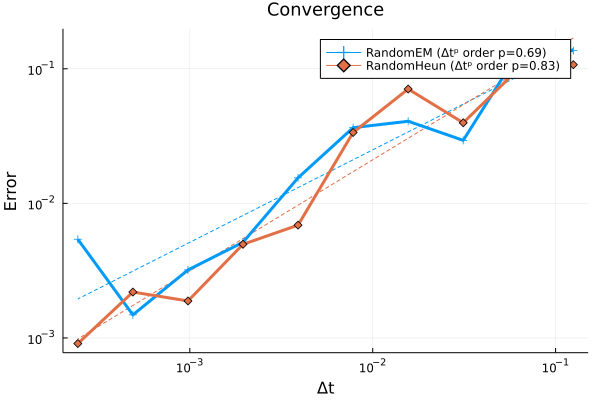
\includegraphics[scale=0.8]{img/plot_13.png}
\end{figure}

For a lower order convergence, below order $1$, we take the noise $\{Y_t\}_t$ to be the transport process defined by
$$
Y_t = \sin(t/Z)^{1/3},
$$
where $Z$ is a beta random variable $Z \sim B(\alpha, \beta)$. Notice $Z$ takes values strictly within $(0, 1)$ and, hence, $\sin(t/Z)$ can have arbitrarily high frequencies and, hence, go through the critic value $y = 0$ extremely often.

\textcolor{red}{(Need to remove the Heun method and do more tests)}.

\section{Estimate on the solution}

We assume $f=f(t, x, y)$ is continuous on all variables and is Lipschitz continuous on each variable, i.e. there exist constants $L_t, L_x, L_y \geq 0$ such that
\begin{align}
  |f(t_1, x, y) - f(t_2, x, y)| & \leq L_t |t_1-t_2|, \\
  |f(t, x_1, y) - f(t, x_2, y)| & \leq L_x |x_1 - x_2|, \\
  |f(t, x, y_1) - f(t, x, y_2)| & \leq L_y |y_1 - y_2|,
\end{align}
for all $t, t_1, t_2 \in I$, $x, x_1, x_2 \in \mathbb{R}$ and $y, y_1, y_2\in \mathbb{R}$. By the continuity of $f=f(t, x, y)$, we also have
$$
M_0 = \sup_{t\in I} |f(t, 0, 0)| < \infty.
$$
These conditions imply that $f$ has an at most linear growth in $x$ and $y$:
\begin{equation}
    \label{Mfestimate}
    |f(t, x, y)| \leq M_0 + L_x|x| + L_y|y|,
\end{equation}
for every $(t, x, y) \in [0, T] \times \mathbb{R} \times \mathbb{R}$.

We assume the initial condition has a bounded first moment:
\begin{equation}
    \label{EX0assumption}
    \mathbb{E}[|X_0|] \leq C_0 < \infty.
\end{equation}

As for the noise, we assume, for now, that
\begin{equation}
    \label{EYtassumption}
    \mathbb{E}[|Y_t|] \leq M_Y, \qquad \forall t\in [0, T].
\end{equation}

With the assumed regularity on $f=f(t, x, y)$, the solutions of \eqref{rodeeq} are pathwise solutions, so that
$$
X_t = X_0 + \int_0^t f(s, X_s, Y_s) \;\mathrm{d}s.
$$

Using \eqref{Mfestimate}, we estimate each solution with
$$
    |X_t|  \leq |X_0| + \int_0^t (M_0 + L_x |X_s| + L_y |Y_s|) \;\mathrm{d}s.
$$
Using Gronwall's lemma, we find
\begin{equation}
    \label{Xtestimate}
    |X_t| \leq \left( |X_0| + M_0 t  + L_y \int_0^t |Y_s| \;\mathrm{d}s\right) e^{L_x t}, \quad t \in [0, T].
\end{equation}
In particular, taking the expectation, 
$$
    \mathbb{E}[|X_t|] \leq \left( \mathbb{E}[|X_0|] + M_0 t  + L_y \int_0^t \mathbb{E}[|Y_s|] \;\mathrm{d}s\right) e^{L_x t}, \quad t \in [0, T].
$$

Using hypotheses \eqref{EX0assumption} and \eqref{EYtassumption}, we find that
$$
\mathbb{E}[|X_t|] \leq \left( C_0 + (M_0 + L_y M_Y) t \right) e^{L_x t}, \quad t \in [0, T].
$$
hence,
\begin{equation}
    \label{EXtestimate}
    \mathbb{E}[|X_t|] \leq M_X, \qquad t \in [0, T],
\end{equation}
with
\begin{equation}
    \label{MXt}
    M_X = (C_0 + (M_0 + L_y M_Y)T)e^{L_x T}.
\end{equation}


Similarly, we write, for $t \geq t_0 > 0$,
$$
X_t - X_{t_0} = \int_{t_0}^t f(s, X_s, Y_s) \;\mathrm{d}s.
$$
Using \eqref{Mfestimate}, we estimate
\begin{align*}
    |X_t - X_{t_0}| & \leq \int_{t_0}^t \left(M_0 + L_x |X_s| + L_y|Y_s| \right)\;\mathrm{d}s \\
    & \leq L_x \int_{t_0}^t |X_s| \;\mathrm{d}s + L_y\int_{t_0}^t |Y_s|\;\mathrm{d}s + M_0(t - t_0).
\end{align*}

Using \eqref{Xtestimate}, we obtain
\begin{equation}
    |X_t - X_{t_0}| \leq L_x \int_{t_0}^t \left( |X_0| + M_0 s  + L_y \int_0^s |Y_\sigma| \;\mathrm{d}\sigma\right) e^{L_x s} \;\mathrm{d}s + L_y\int_{t_0}^t |Y_s|\;\mathrm{d}s + M_0(t - t_0)
\end{equation}

\section*{Appendix}

The heart of the matter is the following. Think of $\tau$ as the time-step $\Delta t$, but we use $\tau$ for simplicity. Let $g=g(t)$ be a $\theta$-H\"older continuous function, with H\"older constant $C$. Then, we can do the usual ``local''-type estimate
\begin{align*}
    \left|\int_0^T \left(g(t + \tau) - g(t) \right) \;\mathrm{d}t \right| & \leq \int_0^T \left|g(t + \tau) - g(t) \right| \;\mathrm{d}t \\
    & \leq C\int_0^T \tau^{\theta} \;\mathrm{d}t \\
    & = C\tau^{\theta}T,
\end{align*}
which yields an order $\theta$ approximation, with respect to the ``time step" $\tau$. However, we can also integrate first, so that
\begin{align*}
    \left|\int_0^T \left(g(t + \tau) - g(t) \right) \;\mathrm{d}t \right| & = \left|\int_0^T g(t + \tau) \;\mathrm{d}t - \int_0^T g(t) \;\mathrm{d}t \right| \\ 
    & = \left| \int_\tau^{T+\tau} g(t) \;\mathrm{d}t - \int_0^T g(t) \;\mathrm{d}t \right| \\
    & = \left| \int_T^{T+\tau} g(t) \;\mathrm{d}t - \int_0^\tau g(t) \;\mathrm{d}t \right| \\
    & \leq 2\max_t|g(t)| \tau,
\end{align*}
which reveals the order 1 convergence, even without assuming that $g$ is H\"older.

For the discretization, however, we don't have $g(t+\tau) - g(t)$, but actually steps $g(t) - g(\tau^N(t))$, where $\tau^N(t)$ picks the largest $j\tau$ smaller than or equal to $t$, i.e. $\tau^N(t) = \max\{j\tau; \; j\tau \leq t, j\}$. And there is also the dependency on the solution $X_t$ itself, leading to the steps $f(t, X_{\tau^N(t)}, Y_t) - f(\tau^N(t), X_{\tau^N(t)}, Y_{\tau^N(t)})$. The idea, then, is to assume that these steps can be bound by
\begin{multline*}
  |f(t, X_{\tau^N(t)}, Y_t) - f(\tau^N(t), X_{\tau^N(t)}, Y_{\tau^N(t)})| \\
  \leq (G_t - G_{\tau^N(t)})h(X_{\tau^N(t)}) + G^0_t - G^0_{\tau^N(t)},
\end{multline*}
where the bounding process $G_t$ (usually $G_t = g(t, Y_t)$ for some $g=g(t, y)$, but not necessarily) is assumed to have monotone nondecreasing sample paths. In this case, an estimate similar to the above can be obtained, and the strong order 1 convergence, achieved.

Keep in mind that assuming that $g(t)$ is the difference of monotone functions, then $g$ is differentiable almost everywhere, but that is not quite the same as saying that it is Lipschitz, not even absolutely continuous nor of bounded variation. Think of that classical example that $g$ is constant almost everywhere, hence $g' = 0$ almost everywhere, and $\int_0^1 g'(s) \;\mathrm{d}s = 0$, but $g(1) > g(0)$. In fact, there is an important case that falls into this category which is the renewal-reward process, that has jump discontinuities and each sample path can be written as the difference between two monotonically nondecreasing jump functions. More general point-process such as the Hawkes process used, e.g. in earthquake models should also work. These are great examples!

\dontshow{For the power function $t \mapsto t^\theta$, for $t \geq 0$, with $0<\theta\leq 1$, we have, for $t > s \geq 0$,
\begin{align*}
    \frac{|t^{\theta} - s^{\theta}|}{|t - s|^\theta} = \frac{\left|1 - \left(\frac{s}{t}\right)^\theta\right|}{\left|1 - \left(\frac{s}{t}\right)\right|^\theta} \leq \frac{\left|1 - \left(\frac{s}{t}\right)\right|}{\left|1 - \left(\frac{s}{t}\right)\right|} = 1,
\end{align*}
where we used that $(s/t)^\theta \geq (s/t)$, since $0 \leq s/t < 1$ and $0 < \theta \leq 1$, and, similarly, that $(1 - s/t)^\theta \geq (1 - s/t)$. This shows that $t \mapsto t^\theta$ is H\"older continuous with H\"older exponent $\theta$ and H\"older constant $1$.
}


\section*{Acknowledgments}


\begin{thebibliography}{25}


\end{thebibliography}

\end{document}